\documentclass[11pt]{article}
\usepackage{textcomp,geometry,graphicx,verbatim}
\usepackage{fancyhdr}
\usepackage{amsmath,amssymb,enumerate,cancel}
\usepackage{titling}
\setlength{\droptitle}{-10em}   % This is your set screw
\pagestyle{fancy}
\def\Name{Manohar Jois}
\def\Homework{3} % Homework number - make sure to change for every homework!
\def\Session{Spring 2015}

% Extra commands
\let\origleft\left
\let\origright\right
\renewcommand{\left}{\mathopen{}\mathclose\bgroup\origleft}
\renewcommand{\right}{\aftergroup\egroup\origright}
\newcommand{\N}{\mathbb{N}}
\newcommand{\Z}{\mathbb{Z}}
\newcommand{\R}{\mathbb{R}}
\newcommand{\Q}{\mathbb{Q}}
\newcommand{\C}{\mathbb{C}}
\newcommand{\p}[1]{\left(#1\right)}
\newcommand{\E}{\mathbb{E}}
\newcommand{\cov}{\text{Cov}}
\newcommand{\lhood}{\mathscr{L}}
\renewcommand{\gcd}[1]{\text{gcd}\p{#1}}
\renewcommand{\deg}[1]{\text{deg}\p{#1}}
\renewcommand{\log}[1]{\text{log}\p{#1}}
\renewcommand{\ln}[1]{\text{ln}\p{#1}}
\newcommand{\logb}[2]{\text{log}_{#1}\p{#2}}
\newcommand{\BigOh}[1]{O\p{#1}}
\newcommand{\BigOmega}[1]{\Omega\p{#1}}
\newcommand{\BigTheta}[1]{\Theta\p{#1}}
\newcommand{\asdf}{\newline\newline}

\title{CS189\ \Session\  --- Homework \Homework\ (2 slip days used)}
\author{\Name}
\lhead{CS189\ \Session\  Homework \Homework\ Problem \theproblemnumber,\ \Name}

\begin{document}
\maketitle
\newcounter{problemnumber}
\setcounter{problemnumber}{0}

\section*{Problem 1}
\stepcounter{problemnumber}
\begin{enumerate}[(a)]
\item (see \texttt{README} and \texttt{p1out.txt})
\item (see \texttt{README} and \texttt{p1out.txt})
\item (see \texttt{README} and \texttt{p1out.txt})
\item 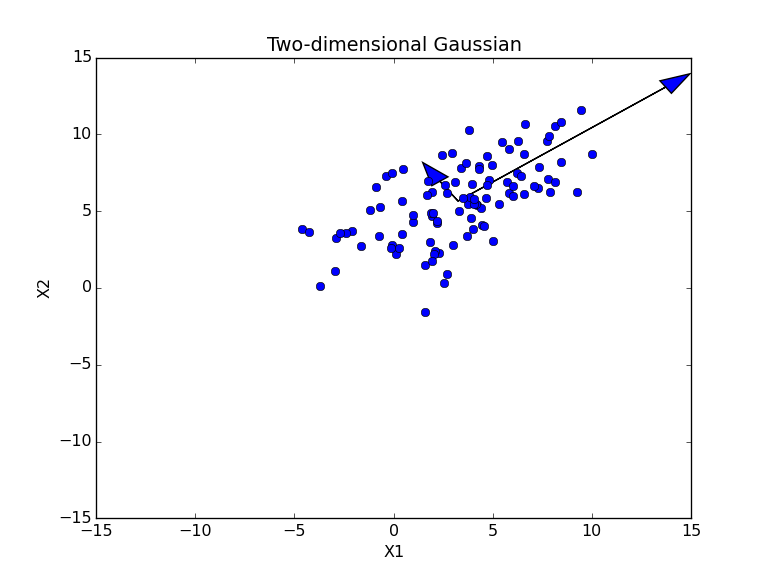
\includegraphics[scale=0.45]{images/p1d}
\item 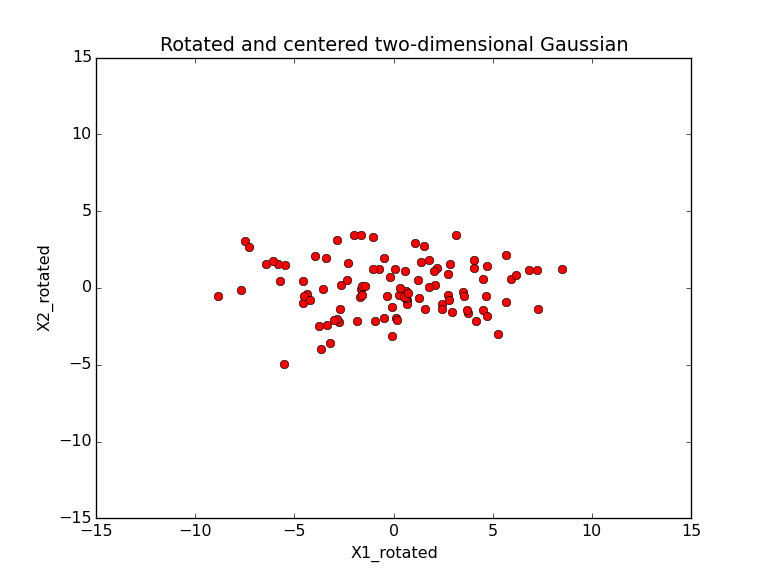
\includegraphics[scale=0.45]{images/p1e}
\end{enumerate}


\newpage
\section*{Problem 2}
\stepcounter{problemnumber}


\newpage
\section*{Problem 3}
\stepcounter{problemnumber}
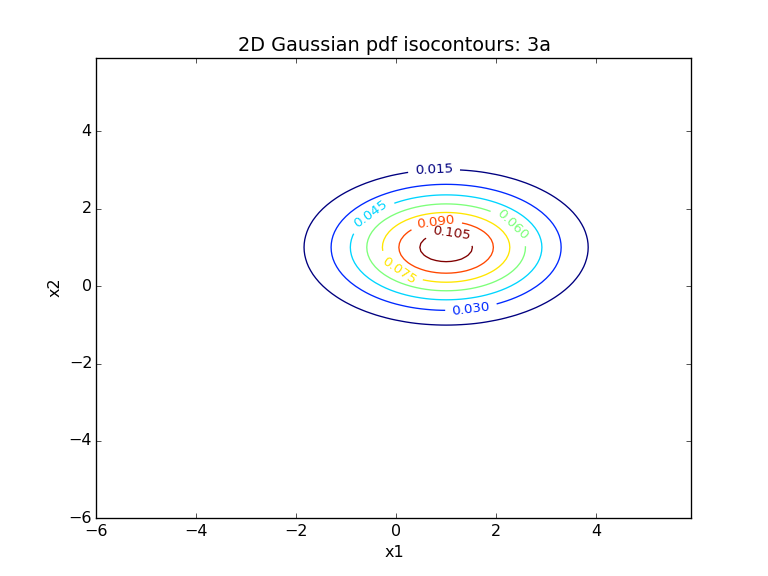
\includegraphics[scale=0.45]{images/p3a}
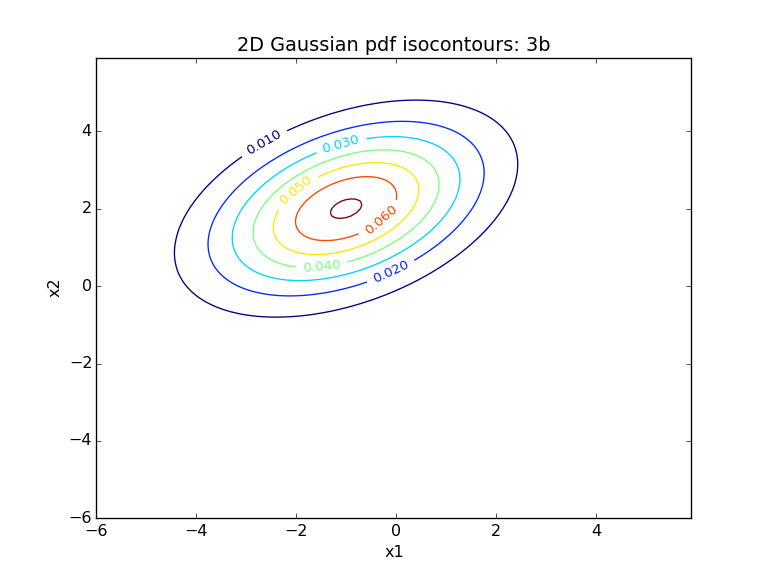
\includegraphics[scale=0.45]{images/p3b}
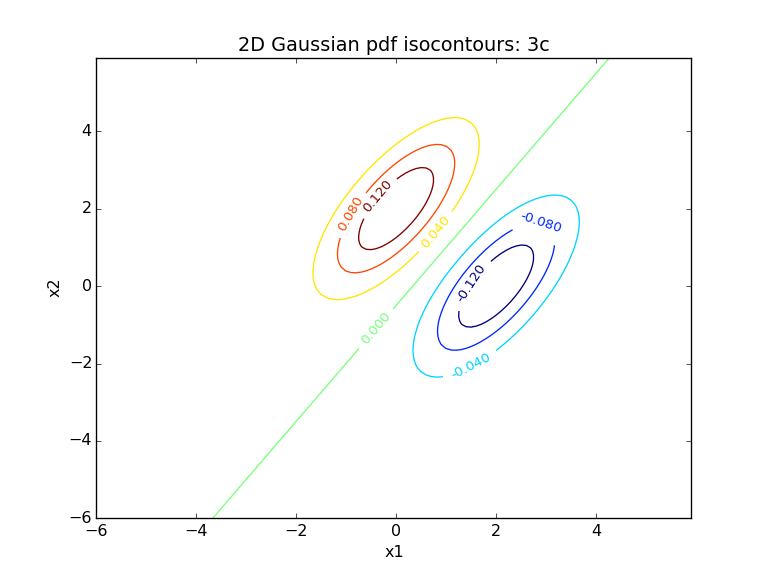
\includegraphics[scale=0.45]{images/p3c}
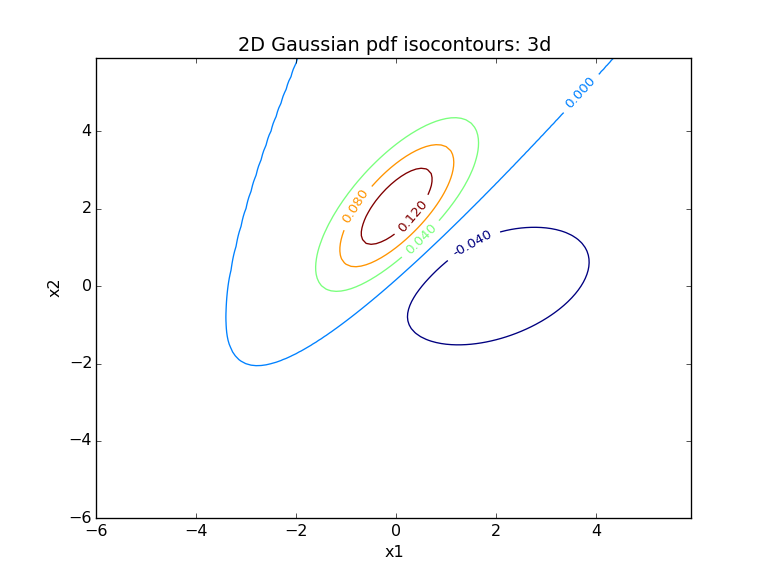
\includegraphics[scale=0.45]{images/p3d}
%\begin{tabular}{cc}
%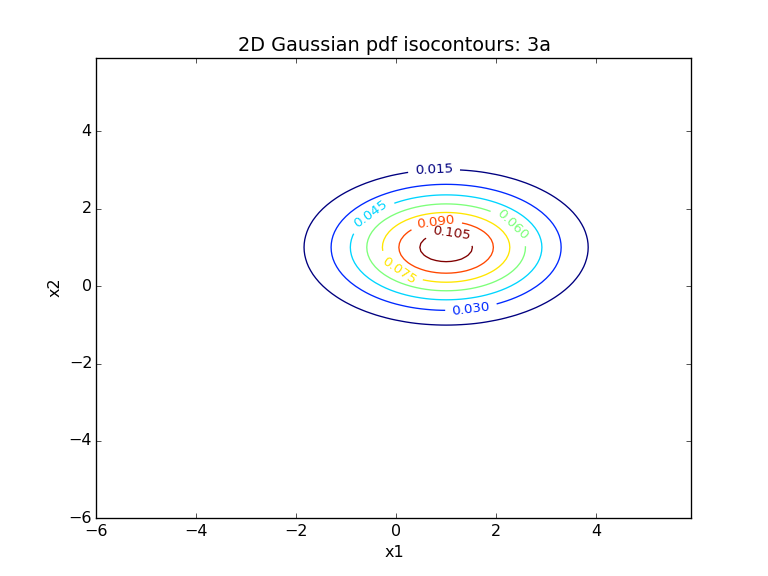
\includegraphics[scale=0.4]{images/p3a} & 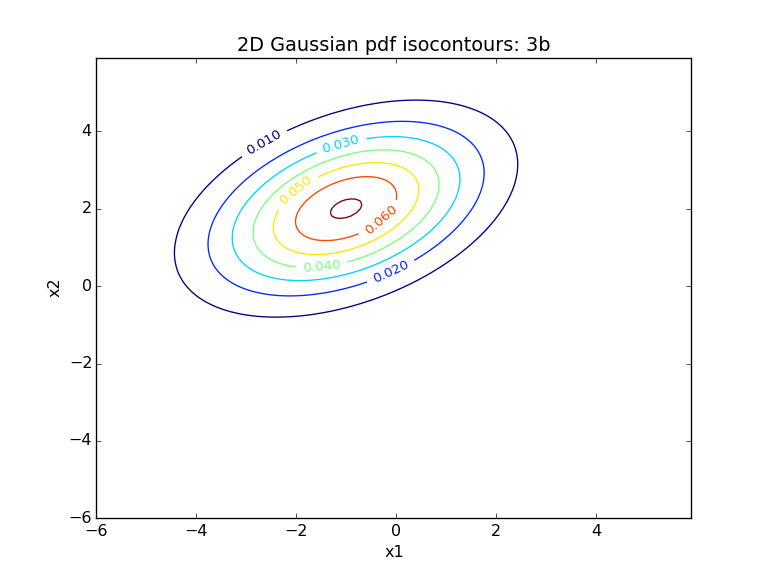
\includegraphics[scale=0.4]{images/p3b} \\
%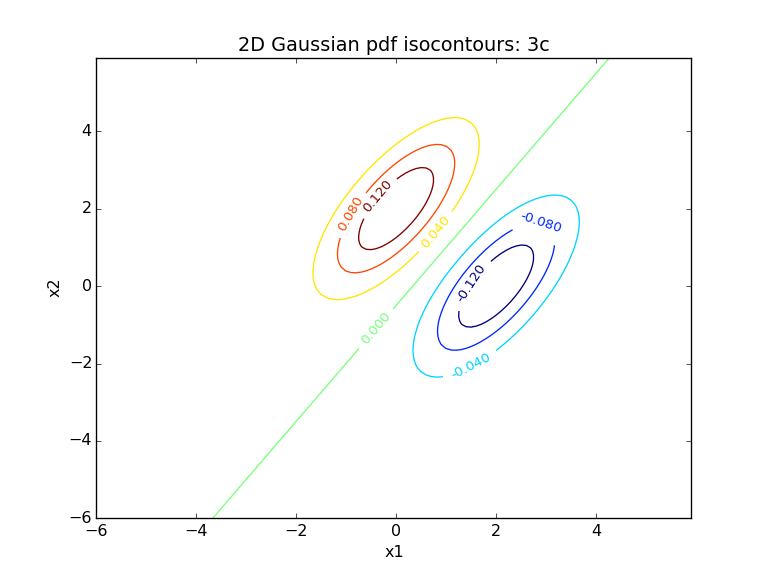
\includegraphics[scale=0.4]{images/p3c} & 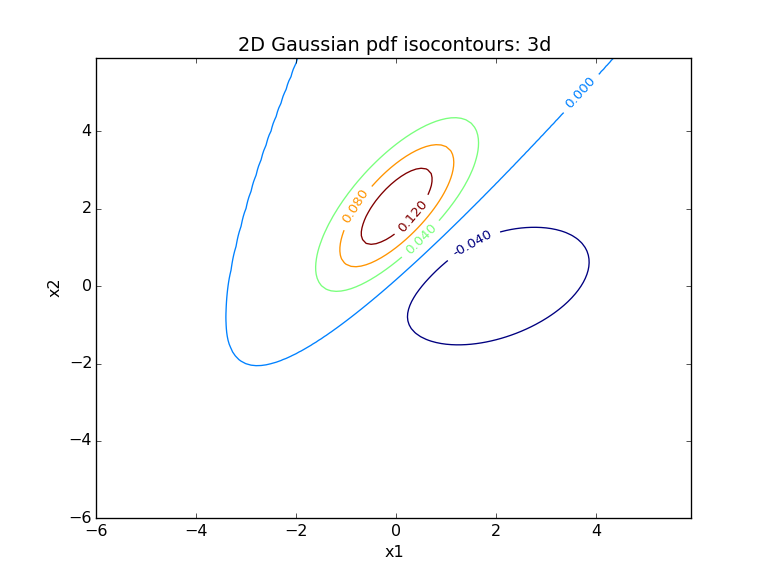
\includegraphics[scale=0.4]{images/p3d} \\
%\end{tabular}
%\newpage
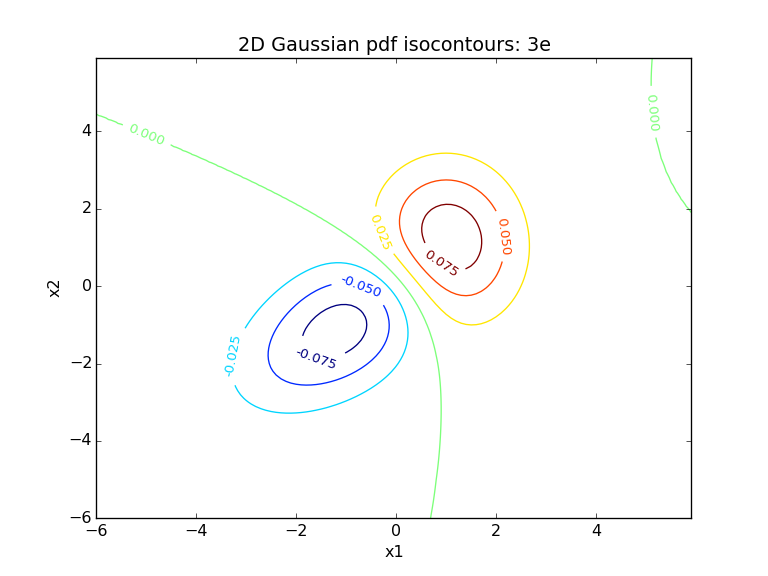
\includegraphics[scale=0.45]{images/p3e}


\newpage
\section*{Problem 4}
\stepcounter{problemnumber}
\begin{enumerate}[a)]
\item 
\item We model the priors as approximately uniform, and indeed the frequencies of each class in the training set are nearly equal. The priors are listed here and in \texttt{p4out.txt}:
\begin{verbatim}
Label: 0        P(Y=0) = 0.0979
Label: 1        P(Y=1) = 0.1125
Label: 2        P(Y=2) = 0.1000
Label: 3        P(Y=3) = 0.1016
Label: 4        P(Y=4) = 0.0979
Label: 5        P(Y=5) = 0.0902
Label: 6        P(Y=6) = 0.0991
Label: 7        P(Y=7) = 0.1039
Label: 8        P(Y=8) = 0.0975
Label: 9        P(Y=9) = 0.0992
\end{verbatim}
\item This is the covariance matrix for the digit class '5':\\
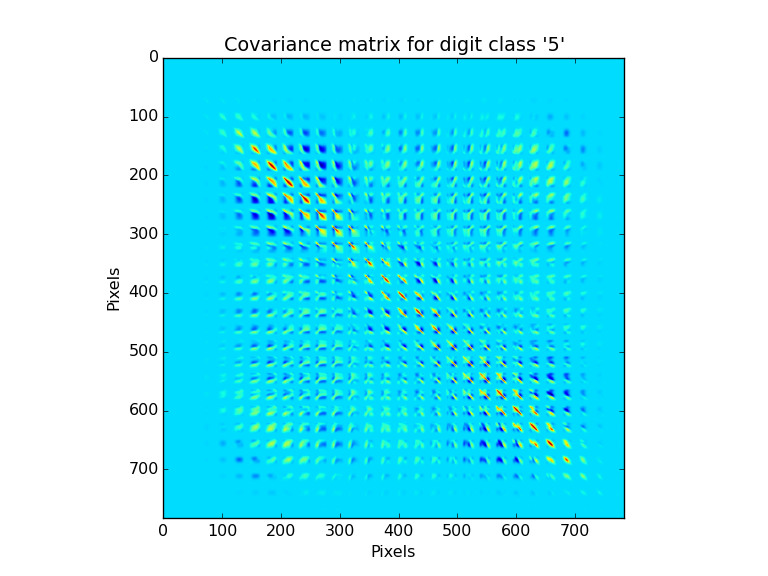
\includegraphics[scale=0.6]{images/p4c}
\newpage
\item 
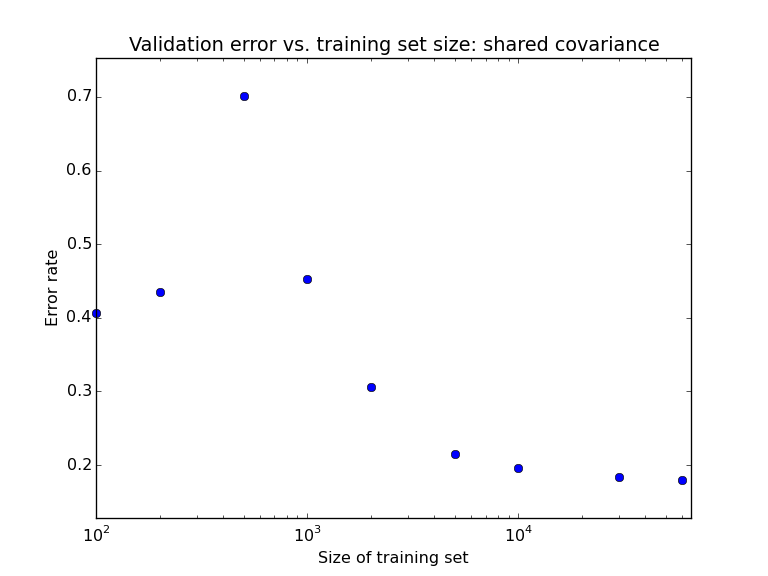
\includegraphics[scale=0.45]{images/p4d1}
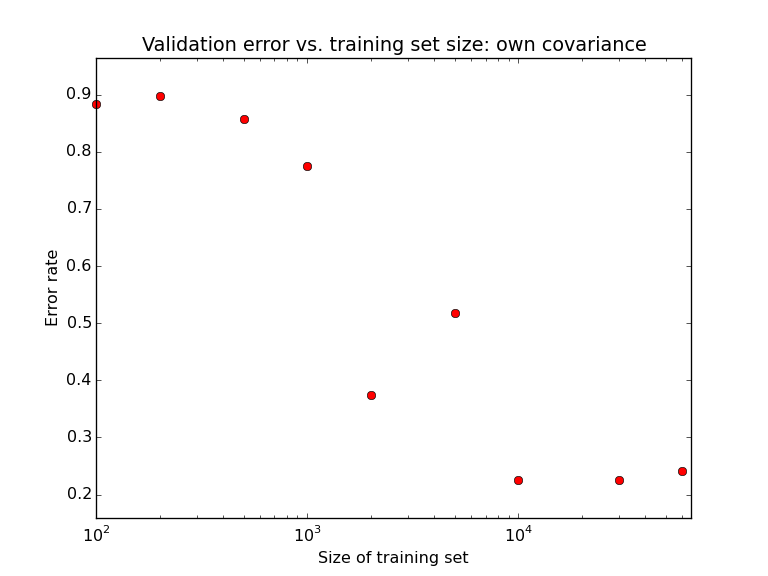
\includegraphics[scale=0.45]{images/p4d2}
Kaggle accuracy for Gaussian digits classifier was $0.83040$
\item Kaggle accuracy for Gaussian spam classifier was $0.81352$
\end{enumerate}


\newpage
\section*{Problem 5}
\stepcounter{problemnumber}
We simply expand the loss function, take the gradient w.r.t. both parameters and solve for when the gradients are zero. This will minimize the loss function because it can be written as the sum of two squared L2 norms, which is convex. The cancellations to zero in the derivation take advantage of the fact that $\sum_i x_i = 0$. \begin{align*}
J(w,w_0) &= (y^T-w^TX^T-w_01^T)(y-Xw-w_01)+\lambda w^Tw\\
&= y^Ty-y^TXw-w_0y^T1-w^TX^Ty+w^TX^TXw+w_0\cancelto{0}{w^TX^T1}-w_01^Ty+w_0\cancelto{0}{1^TXw}+w_0^21^T1+\lambda w^Tw\\
&= y^Ty-y^TXw-w^TX^Ty+w^TX^TXw-2\sum_iw_0y_i+nw_0^2+\lambda w^Tw
\end{align*}
Solving for the optimal $\hat{w_0}$:
\begin{align*}
\nabla_{w_0}J &= 2nw_0-2\sum_iy_i = 0\\
n\hat{w_0} &= \sum_iy_i\\
\hat{w_0} &= \frac1n\sum_iy_i = \bar{y}
\end{align*}
Solving for the optimal $\hat{w}$:
\begin{align*}
\nabla_wJ &= -X^Ty-X^Ty+2X^TXw+2\lambda Iw = 0\\
(X^TX+\lambda I)\hat{w} &= X^Ty\\
\hat{w} &= (X^TX+\lambda I)^{-1}X^Ty
\end{align*}


\newpage
\section*{Problem 6}
\stepcounter{problemnumber}
Maximizing the likelihood of $w_0,w_1$ given $y,x$ is equivalent to maximizing $P(y,x|w_0,w_1)\propto P(y|x,w_0,w_1)\propto P(y|x)$ (uniform priors). Because the samples are drawn independently, $P(y|x)=\prod_i P(y_i|x_i)$ and we can maximize this to maximize likelihood:
\begin{align*}
\ell(w_0,w_1) &= \prod_{i=1}^n\frac1{\sigma\sqrt{2\pi}}\exp\left(\frac{-(y_i-(w_0+w_1x_i))^2}{2\sigma^2}\right)\\
\ln{\ell} &= \sum_{i=1}^n-\ln{\sigma\sqrt{2\pi}}-\left(\frac{-(y_i-w_1x_i-w_0)^2}{2\sigma^2}\right)\\
\frac{\partial\ln{\ell}}{\partial w_0} &= \sum_{i=1}^n-\frac1{\sigma^2}(y_i-w_1x_i-w_0)(-1) = 0\\
nw_0 &= \sum_{i=1}^ny_i-w_1\sum_{i=1}^nx_i\\
w_0 &= \bar{y}-w_1\bar{x}
\end{align*}
We can plug in the optimal $w_0$ into the log-likelihood to solve for the optimal $w_1$:
\begin{align*}
\ln{\ell} &= \sum_{i=1}^n-\ln{\sigma\sqrt{2\pi}}-\left(\frac{-((y_i-\bar{y})-w_1(x_i-\bar{x}))^2}{2\sigma^2}\right)\\
\frac{\partial\ln{\ell}}{\partial w_0} &= \sum_{i=1}^n-\frac1{\sigma^2}((y_i-\bar{y})-w_1(x_i-\bar{x}))(-(x_i-\bar{x})) = 0\\
w_1\sum_{i=1}^n(x_i-\bar{x})^2 &= \sum_{i=1}^n(x_i-\bar{x})(y_i-\bar{y})\\
w_1 &= \frac{\sum_i(x_i-\bar{x})(y_i-\bar{y})}{\sum_i(x_i-\bar{x})^2}
\end{align*}


\newpage
\section*{Problem 7}
\stepcounter{problemnumber}
\begin{enumerate}[(a)]
\item The example $P(X=0) = 1/2 \neq P(X=0|Y=0)=0$ (and vice versa for $Y$) clearly shows $X$ and $Y$ are not independent. Also, by symmetry, $\E[X] = \E[Y] = 0$ and therefore $\cov(X,Y)=\E[(X-\E[X])(Y-\E[Y])] = \E[XY] = 0$ since all outcomes must have one of them equal to zero. Thus $X$ and $Y$ are uncorrelated.
\item Consider $X$ and $Y$. Knowing the value of $Y$ only tells you whether $B_2$ and $B_3$ are equal or different, and within both those events, $B_2$ still retains a uniform distribution over its domain $\{0,1\}$. In either case, $B_1$ is still equally likely to be equal to or different from $B_2$, and so the distribution of $X$ doesn't change whether we know $Y$ or not (still a 50-50 split). By symmetry, the same argument holds for $(X,Z)$ and $(Y,Z)$, so they are pairwise independent.\asdf
However, note that $P(X=1)=1/2 \neq P(X=1|Y=1,Z=1)=0$ because the latter means $B_3$ is different from both $B_1$ and $B_2$, which necessarily implies $B_1=B_2$. It is not always true that $P(X)=P(X|Y,Z)$ and by symmetry the same goes for $P(Y|X,Z)$ and $P(Z|X,Y)$, so the three variables are not mutually independent.
\end{enumerate}

\end{document}
